\documentclass{jsarticle}
\usepackage[margin = .7in]{geometry}
\usepackage[dvipdfmx]{graphicx}
\usepackage{listings}
\usepackage{amsmath}
\usepackage{bm}
\usepackage{ascmac}
\lstset{%
  language={python},
  basicstyle={\small},%
  identifierstyle={\small},%
  commentstyle={\small\itshape},%
  keywordstyle={\small\bfseries},%
  ndkeywordstyle={\small},%
  stringstyle={\small\ttfamily},
  frame={tb},
  breaklines=true,
  columns=[l]{fullflexible},%
  numbers=left,%
  xrightmargin=0zw,%
  xleftmargin=3zw,%
  numberstyle={\scriptsize},%
  stepnumber=1,
  numbersep=1zw,%
  lineskip=-0.5ex%
}

\begin{document}
\title{卒論テーマ候補 :ゆびすま}
\author{池上 慧}
\maketitle

\section{「ゆびすま」とは}
「ゆびすま」とは2人以上で行われるゲームである。ここでは2人で行われるケースを想定する。プレイヤーは毎回「攻め」と「守り」の役目を交互に行う。プレイヤーは毎回好きな本数の親指を上げる。「攻め」のプレイヤーは今回上がる親指の本数を予想し、掛け声とともにその予想した数をコールしながら、自分でも好きな本数だけ親指を上げる。「守り」のプレイヤーは掛け声の後に親指を好きな本数だけあげる。「攻め」がコールした数と実際にあげられた親指の総数が等しかったなら「攻め」の勝ちであり、そうでなければ「引き分け」である。引き分けたら役割を交代してどちらかが勝つまで続けるものとする。(本来であれば勝てば腕を一本減らすことができ、先に二回勝利した方の勝ちというルールであるが、ここでは最初の一回の勝利が起こるまでの、2本vs2本の状況のみを想定する。)

以下ではコールできる指の本数を2までに限定した「限定ゆびすま」をまずは考える。このルールのもとでは、守り手の行動を$\left\{ 0,1,2 \right\}$だと正しく認識した場合に、混合戦略ナッシュ均衡で各アクションに割り振られる確率に大小が生じる。一方で後に提示する「通常ゆびすま」ではコールできる指の本数を4本まで許容していて、このルールのもとでは正しい認識を持った時、勝つ可能性のある手に振られる確率は全て等しくなる。この二つのルールによる差を何かに使えないか?

\section{研究の意図するところ}
ゆびすまで攻め手の戦略を決める肝は、「自分のコールと自分で揚げる親指の数の差」であることは明らかである。ここで「$a$とコールしながら$b$本の親指を上げる」という行動を$(a,b)$と表記することにすると、$\left\{ (0,0), (1,1), (2,2)\right\}$は自分のコールと自分のゆびの数が等しい組(set1)で、$\left\{ (1,0), (2,1)\right\}$を自分のコールが自分のゆびの数よりも1つ多い組(set2)、$\left\{ (2,0)\right\}$を自分のコールが自分のゆびの数よりも2つ多い組(set3)の3つに戦略を分類することができる。

これらはそれぞれ同じ組の中では勝利確率は等しい。以下で計算するように、相手の戦略を$\left\{ 0,1,2\right\}$、すなわちゆびを上げる本数だと捉えると、この全てをサポートに持つ混合戦略ナッシュ均衡がこのゲームの唯一のナッシュ均衡として存在し、その時以上のセットには全て等確率、すなわち$\frac{1}{3}$ずつの確率が振られることになる。この時、各セットに含まれる戦略の数は異なっていることに注意すると、個別の戦略に振られる確率はset3の中身、set2の中身、set1の中身の順番で大きくなるはずである。

しかし、この結果は直感に反するものである。$\left\{ (2,0)\right\}$を選ぶということは自分は1本も上げないで、相手が2本とも上げることを想定しているということであるが、これが実現する可能性は低そうに思えてしまう。実際、何も説明せずに友人とこのゲームを繰り返し行った時、いきなり$\left\{ (2,0)\right\}$が選ばれる回数は少なかった。

むしろ選ばれがちなのはset2、すなわち$\left\{ (1,0), (2,1)\right\}$の2つであった。本研究ではゆびすまにおいてset2が戦略として選ばれやすいことの理由として、「攻め手が知らず知らずのうちに守り手の左右の手を別々の意思決定主体が操作するものだと想定してゲームをプレイしている」という仮説を検証する。

以下で計算するように、守り手の腕を別々の主体と想定した場合の混合戦略ナッシュ均衡は現実的なものが3つ存在し、そのどれもでset2に高い確率が付与されている。逆にset1やset3には確率が付与されない均衡も存在し、それらの戦略を極端な手として嫌ってしまう傾向と合致していると言える。

さらに限定合理性の文脈で提案されている各種解概念との比較を行うことで、限定合理性の一形態として相手主体の誤認があり得ることを確認する。

\section{限定ゆびすまのナッシュ均衡}
計算は別紙。

$(q, r, s)$でcase1において守り手が$\left\{ 0,1,2\right\}$をそれぞれ取る確率を、$p$でcase2において守り手の左右の腕が取る混合戦略、すなわち親指を上げる確率を、$(x, y, z)$で攻め手が取る混合戦略、すなわちset1, set2, set3をとる確率を表すとする。この時、それぞれのケースでいかが混合戦略ナッシュ均衡となる。

\begin{itembox}[l]{case1 : 相手が統一された意思決定主体だと想定}
    \begin{align}
    	\begin{cases}
		(q, r, s) = (\frac{1}{3}, \frac{1}{3}, \frac{1}{3})\\
		(x, y, z) = (\frac{1}{3}, \frac{1}{3}, \frac{1}{3})
	\end{cases}
    \end{align}
\end{itembox}

\begin{itembox}[l]{case2 : 相手の左右の手を別々の意思決定主体だと想定}
\begin{align}
    	&\begin{cases}
		p = \frac{1}{3}\\
		(x, y, z) = (\frac{1}{3}, \frac{2}{3}, 0)
	\end{cases}\\[10pt]
	&\begin{cases}
		p = \frac{1}{2}\\
		(x, y, z) = (0, 1, 0)
	\end{cases}\\[10pt]
	&\begin{cases}
		p = \frac{2}{3}\\
		(x, y, z) = (0, \frac{2}{3}, \frac{1}{3})
	\end{cases}
\end{align}
\end{itembox}

\section{データへのフィットの比べ方}
ゆびすまを実際に対戦させてデータを集めることを想定する。そのデータに対して先の二つのモデルの説明度合いを比較してどちらのモデルが採択されるかを調べたい。単純に考えられるのは以下のように尤度を比較すること。

case1に対しては通常の意味で対数尤度が計算できる。case2に対しては以下のようにEMアルゴリズムを用いてその対数尤度を計算する。
$i = 1, \dots, n$を$n$回のプレイのindexとする。$Y_i$を攻め手が$i$回目のプレイで行った戦略を示す確率変数であるとする。すなわちそのサポートは$\left\{ (0,0), (1,1), (2,2), (1,0), (2,1), (2,0)\right\}$の6つである。$j = 1, 2, 3$で均衡のindexとして、それぞれ先の均衡(2), (3), (4)を示すとする。この時、$f_j(y_i)$は均衡$j$がプレイ$i$で実現している時に、攻め手が出す戦略の確率分布関数である。先に定義された戦略のset内では均等に確率が分配されるとすると、それぞれ以下のようになる。
\begin{align}
	f_1(y_i) = \begin{cases}
			\frac{1}{9} & y_i \in \text{set1}\\[8pt]
			\frac{1}{3} & y_i \in \text{set2}\\[8pt]
			0 & y_i \in \text{set3}
		\end{cases}\qquad
	f_2(y_i) = \begin{cases}
			0 & y_i \in \text{set1}\\[8pt]
			\frac{1}{2} & y_i \in \text{set2}\\[8pt]
			0 & y_i \in \text{set3}
		\end{cases}\qquad
	f_3(y_i) = \begin{cases}
			0 & y_i \in \text{set1}\\[8pt]
			\frac{1}{3} & y_i \in \text{set2}\\[8pt]
			\frac{1}{3} & y_i \in \text{set3}
		\end{cases}
\end{align}

ここで均衡$j$が選ばれる確率を$\psi_j$で書くとすると、$Y_i$は混合分布である$\sum_j \psi_j f_j(y_i)$に従うとできる。missing variableとして各プレイがどの均衡から生じたものなのかを示した確率変数$u_i$を考えると、完全なデータが与えられた時の尤度は、$I(\cdot)$を指示関数とすると以下のように書ける。
\begin{align}
	L(Y, u | \psi) = \Pi_i\ \Pi_j\ (\psi_j\cdot f_j(y_i))^{I(u_i = j)}
\end{align}

Q関数の定義は以下である。
\begin{align*}
	Q(\psi | \psi^{(0)}) = E_{\psi^{(0)}}\left[ {\rm log}\ L(Y, u | \psi)\ |\ Y \right]
\end{align*}

Q関数はパラメータについて最大化されるので、パラメータに関連する部分だけ残せば最大化のための一階条件を問題なく得られる。従って以下では$\psi$に関係のない項は省略してイコールで記す。ただし、$\psi^{0}$はEMアルゴリズムないで一回前のiterationで得られたパラメータの値であり、期待値はmissing variableについて取られているとする。
\begin{align}
	E_{\psi^{(0)}}\left[ {\rm log}\ L(Y, u | \psi)\ |\ Y \right] &= \sum_i \sum_j E_{\psi^{(0)}}\left[ I(u_i = j) {\rm log}\ \psi_j\ |\ Y \right]\nonumber \\
	&= \sum_j {\rm log}\ \psi_j\ \sum_i E_{\psi^{(0)}}\left[ I(u_i = j)\ |\ Y \right]
\end{align}

これをパラメータ$\psi_1, \psi_2, \psi_3$について最大化することを考える。一階条件より
\begin{align}
	\psi_j = \frac{1}{n} \sum_i E_{\psi^{(0)}}\left[ I(u_i = j)\ |\ Y \right]
\end{align}
である。

ここで、ベイズの公式より
\begin{align*}
	E_{\psi^{(0)}}\left[ I(u_i = j)\ |\ Y \right] = P_{\psi^{(0)}}( u_i = j\ |\ Y ) = \frac{p_{\psi^{(0)}} (y_i\ |\ u_i = j) \cdot p_{\psi^{(0)}} (u_i = j)}{p_{\psi^{(0)}} (y_i)} = \frac{f_j(y_i) \cdot \psi_j^{(0)}}{\sum_j \psi_j^{(0)} f_j(y_i)}
\end{align*}
を得るので、先の結果と合わせることでパラメータの更新式として以下を得る。
\begin{align}
	\forall j \quad \psi_j^{(1)} = \frac{1}{n} \sum_i \frac{f_j(y_i) \cdot \psi_j^{(0)}}{\sum_j \psi_j^{(0)} f_j(y_i)}
\end{align}

これによって収束させたパラメータについて先のQ関数の値を計算し、それを持ってcase2の対数尤度とする。case1の対数尤度とcase2のQ関数の値を比較してモデルのフィットを比べる。

\section{通常ゆびすまのナッシュ均衡}
先の限定ゆびすまの時と導かれる混合戦略ナッシュ均衡における各行動集合に割り振られる確率は同じである。守り手についても同様の確率を付与する混合戦略がナッシュ均衡となっている。しかし、通常ゆびすまにおいては先に置いたsetがそれぞれset1が$\left\{ (0,0), (1,1), (2,2)\right\}$、set2が$\left\{ (1,0), (2,1), (3,2)\right\}$、set3が$\left\{ (2,0), (3,1), (4,2)\right\}$となり、集合ないの要素の数が同じであるため、各行動に割り振られる確率自体は限定ゆびすまと異なる。データへのフィットの計算も同様に行えるが、確率関数は限定ゆびすまの時と異なるものとなるので注意が必用。

\section{守り手のデータを活用する}
今までの話は全て攻め手の戦略について注目してきた。データのフィットも攻め手のとった行動に関してのデータのみで行えるものである。しかし守り手の行動を観察することで、「相手の意思決定主体を誤って認識してしまう」という現象が無意識に起こっているか自覚の下で起こっているのかを判断することができるかもしれない。

攻め手がわのデータを用いて、攻め手が守り手の指を別々のものとしてみているというモデルが支持された状況を考える。この時、守り手のとった行動のデータからcase1のモデル、すなわち攻め手が意思決定主体を正しく認識している時のモデルが支持されたとすると、意思決定主体を誤ってしまうのは自分がせめてになった時のみであり、守り手になった時には相手が自分の意思決定主体が統一されていることを理解した上で行動していることを想定していることになる。これはつまり自分が守り手である時は、自分が攻め手に成った時には守り手の意思決定主体を正しく認識して行動するであろうと思っているということを意味する。この場合には意思決定主体の誤認は攻め手に成った時に無意識化でなされている現象だということができるであろう。

守り手がわのデータのフィットを見るのは攻め手がわのデータを用いたものと同様にして行う。(ゆえに同様に妥当性を考えないといけない。)

\section{alternative models}
ナッシュ均衡以外の解を考える。2人完備情報ゲームに対して適用できる解概念として、Osborn and Rubinshtein (1998)で提案されたS(k) EquilibriumやMcKelvey and Palfrey (1995)で提案されたquantal response equilibriumなどがある。しかし、先のように攻め手のアクションとして、勝利できる相手の本数別に行動の組をくくった時点で、そのゲームは2人対称ゼロサムゲームとなる。具体的にそのゲームの利得表は以下のようである。
\begin{figure}[h]
    \centering
    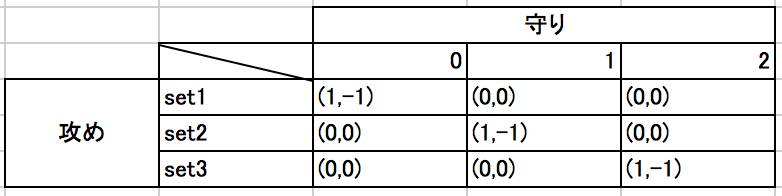
\includegraphics[width=10cm]{pmat.png}
    \caption{利得表}
\end{figure}
このような利得構造を持つゲームにおいては、既存の限定合理性に基づく均衡概念では、想定されるようなset2に偏った分布は道ミクことはできない。

従って、対抗するモデルとして考える限定合理性は、自分の行動のうちでどれとどれが無差別なものであるかを認識するそのあり方に置かれるべきであることわかる。ここである二つの行動が攻め手にとって無差別であるとは、その二つの行動を取った時の利得が全く同じであることを意味している。以上より本研究で対立するモデルは以下の4つとできる。

\begin{description}
	\item[モデル1] 相手主体を正しく認識し利得構造も正しく把握している
	\item[モデル2] 相手主体を誤って認識しているが利得構造は正しく把握している
	\item[モデル3] 相手主体は正しく認識しているが利得構造を誤認している
	\item[モデル4] 相手主体を誤って認識し利得構造も誤認している
\end{description}

ここまで述べてきたのは利得構造は正しく把握しているモデル1とモデル2についてである。以下では利得構造の誤認という意味での限定合理性をどのようにモデルに取り入れるかを考えるが、誤差項を加えるようなランダムな誤認の仕方ではとる行動の分布に偏りが出る状況を記述するのは難しく、またゆびすまのような単純な利得構造において実際の報酬に対しての誤認というのは考えにくい。ここで述べている「利得構造の誤認」はつまるところ「どの戦略が同程度に勝ちやすく、勝ちやすさにはどの程度違いがあるか」についての誤認である。そこで、ゆびすまの攻め手のとる行動が「宣言」と「あげる指の数」という二つの要素から構成されていることに注目し、別の方向性からある戦略の勝ちやすさについての誤認が生まれる状況を記述することを考える。

通常ゆびすまのケースを考える。この時攻め手の行動は以下のような表の上に置くことができる。
\begin{figure}[h]
    \centering
    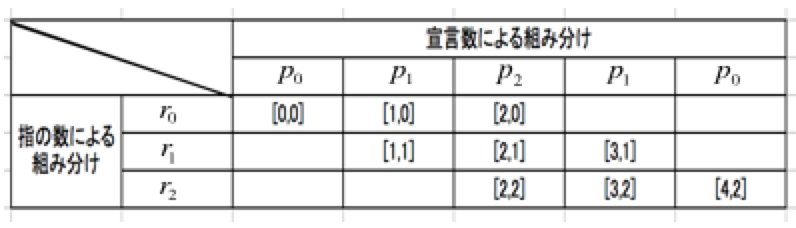
\includegraphics[width=10cm]{class.png}
    \caption{組み分け}
\end{figure}
これは列方向には宣言数で分割し、行方向にはあげるゆびの数で分割したものである。本来は宣言数とゆびの数のペア、このケースでは9ペア、が攻め手の行動として定義されているが、このような複数の手段の組み合わせを一つの行動として見なすのは人間の認知上困難であることが考えられる。その時とられていると認知的過程として、組み合わせを構成する各要素について別々に決定し、それぞれがうまく連携するように行動を決める過程をここでは想定する。すなわち、「勝ちやすい宣言数の選び方」と「勝ちやすいゆび数の選び方」がお互いに矛盾しないように決定され、その積として図2上に配置された本来の戦略が取られる確率が決定される、という状況を考えてみる。

まずモデル3のケース、すなわち相手主体を正しく認識し相手の取りうる行動は$\left\{0,1,2\right\}$のいずれかであると考えているケースを扱う。宣言数について取りうる行動の組は$\left\{ 0,1,2,3,4\right\}$の5つであるが、対称性より守り手は指の本数$0,2$については無差別であるので、攻め手の宣言数については$\left\{ 0,4 \right\},\left\{ 1,3 \right\},\left\{ 2\right\} $がそれぞれ無差別な行動の組となる。したがって、均衡下に置いてはそれぞれに置く確率が等しくなるはずなので、図2のように各宣言数に均衡確率$(p_0, p_1, p_2)$を置く。ただし$2p_0 + 2p_1 + p_2 = 1$であることに注意する。あげる指の数についても対称性を利用して同様に考えることができる。すなわちあげる指の数については$\left\{ 0,2 \right\}, \left\{ 1 \right\}$が無差別な行動の組であり、それぞれに図2のように確率$(r_0, r_1)$を割り振る。ここで$2r_0 + r_1 = 1$であることに注意する。

宣言数サイドと指の数サイドで別々に混合戦略ナッシュ均衡を求めることを考える。ただし、内部でお互いの均衡確率を利用するスキームを用い、お互いが連携するような均衡をいっぺんに求めることを考える。宣言数サイドから具体的に見ていく。守り手の各行動に紐付いた期待損は以下のように書ける。
\begin{align*}
	&\text{expected payoff when the saver chooses 0} = p_0 + \frac{r_1}{r_0 + r_1}p_1 + r_0p_2\\
	&\text{expected payoff when the saver chooses 1} = \frac{r_0}{r_0 + r_1}p_1 + r_1p_2 + \frac{r_0}{r_1 + r_0}p_1\\
	&\text{expected payoff when the saver chooses 2} = r_0p_2 + \frac{r_1}{r_1  + r_0}p_1 + p_0
\end{align*}

ここで$\frac{r_0}{r_0+r_1}$は攻め手が$1$を宣言した時に、指の数サイドの持つ均衡選択確率に従って守り手が負けるケースが実現する条件付き確率である。指の数サイドでの均衡を求める時に必要となる分数も同様の意味での条件付き確率である。守り手がすべての手をサポートに入れた均衡を考えると上記の全てが等しくなる必要がある。

同様に指の数サイドについても期待損を考えると
\begin{align*}
	&\text{expected payoff when the saver chooses 0} = \frac{p_0 + p_2}{p_0 + p_1 + p_2}r_0 + \frac{p_1}{2p_1 + p_2}r_1\\[8pt]
	&\text{expected payoff when the saver chooses 1} = \frac{2p_1}{p_0 + p_1 + p_2}r_0 + \frac{p_2}{2p_1 + p_2}r_1\\[8pt]
	&\text{expected payoff when the saver chooses 2} = \frac{p_0 + p_2}{p_0 + p_1 + p_2}r_0 + \frac{p_1}{2p_1 + p_2}r_1
\end{align*}
であるので、守り手がすべての手をサポートに入れる均衡を考えるとこちらも同じように全てが等しくなる必要がある。

さらに、最終的に得たい混合戦略は図2上の確率分布であるので、和が1となるように制約を課す。以上をまとめると、求める均衡を更生する各サイドの均衡確率は以下の連立方程式の解である。

\begin{align*}
	\begin{cases}
		(r_0 + r_1)p_0 + (r_1 - 2r_0)p_1 + (r_0^2 - r_1^2)p_2&= 0\\
		(p_0 + p_2 - 2p_1)(2p_1 + p_2)r_0 + (p_1 - p_2)(p_0 + p_1 + p_2)r_1 &= 0\\
		2(p_0r_0 + p_1r_0 + p_1r_1 + p_2r_0) + p_2r_1 &= 1\\
		r_1 + 2r_0 &= 1\\
		2p_0 + 2p_1 + p_2 &= 1
	\end{cases}
\end{align*}

上の方程式の解は$(r_0, r_1,p_0, p_1, p_2) = (0, 1, 0, \frac{1}{3}, \frac{1}{3})$である。(pythonによる数値計算)

これでは理論上でないはずの戦略が取られてしまうので、二つの行動間の連携をなくしてみる。これは上の均衡の前に計算してたやつ。

\section{考えたいこと}
\begin{itemize}
	\item 「相手の意思決定に関する勘違いが最適な選択からずれた行動を誘導する」事例としては面白いと思うが、ゆびすまという文脈が陳腐すぎる気がする。どのような書き方をすれば面白くなるか。
	\item 「自分の行動が複数の要素の組み合わせで決定されている時に正しく自分の選択肢を認識できないケース」という事例は面白いお思うが、ゆびすまという例が陳腐すぎる。どういう書き方、文脈の位置付けを行えば面白くなるか。
	\item 無差別な戦略の組をくくる際に起きるミスを扱った限定合理性のモデルはあるか。
	\item 最後の連立方程式が解けない。
	\item 限定ゆびすまでは通常のゆびすまと異なり正しい認識の下でも最適な戦略の導く行動の分布に偏りがある。この違いを面白い形で利用できないか。
\end{itemize}


\end{document}




















